\documentclass[10pt]{article}
\usepackage{uppal}
\usepackage{amssymb}
\usepackage{mathtools}

\begin{document}
\begin{center}
    MAT185H1S - Linear Algebra \\ 
    Winter 2021
\end{center}
Notes on Linear Differential Equations with Constant Coefficients (Part II):

\begin{definition}
    A system of the form
    \vspace{2mm}
    \begin{align*}
        x_1'(t) &= a_{11}x_1(t) + a_{12}x_2(t) + \cdots + a_{1n}x_n(t),& x_1(0)=b_1 \\ 
        x_2'(t) &= a_{21}x_1(t) + a_{22}x_2(t) + \cdots + a_{2n}x_n(t),& x_2(0)=b_2 \\ 
        & \vdots & \\ 
        x_n'(t) &= a_{n1}x_1(t) + a_{n2}x_2(t) + \cdots + a_{nn}x_n(t),& x_n(0)=b_n \\
    \end{align*}
    where each $x_i(t)$ is real-valued function of a real variable, is called a \term{system of linear differential equations with constant coefficients.}
\end{definition}

Writing $\b{x}(t) = \begin{bmatrix}
    x_1(t) \\ x_2(t) \\ \vdots \\ x_n(t)
\end{bmatrix}$, a vector-valued function of $t$, and $A=[a_{ij}]$ for the matrix of the coefficients of the system, we may represent the system as
\begin{equation*}
    \b{x'}=A\b{x},\quad \b{x}(0)=\b{x}_0
\end{equation*}
\vspace{2mm}

Extrapolating our observations and results from the $2\times 2$ case, we give a solution in the case where $A$ is diagonalizable.

\begin{lemma}
    Let $a$ be an $n \times n$ matrix. If $\b{x}_0$ is an eigenvector of $A$ with eigenvalue $\lambda$, then the system $\b{x}'=A\b{x},\, \b{x}(0)=\b{x}_0$ has solution $\b{x}(t)=e^{\lambda t}\b{x}_0$.
\end{lemma}
This lemma yields:
\begin{theorem}
    Let $A$ be a $n\times n$ diagonalizable matrix with eigenvalues $\lambda_1, \lambda_2, \dots, \lambda_n$ (not necessarily distinct). Let $\b{v}_1, \b{v}_2, \dots, \b{v}_n$ be a basis for $\mathbb{R}^n$ consisting of eigenvectors of $A$. If $\b{x}_0 = c_1\b{v}_1 + c_2\b{v}_2+\cdots +c_n\b{v}_n,$ then the system $\b{x}'=A\b{x},\, \b{x}(0)=\b{x}_0$ has solution
    \begin{equation}
        \b{x}(t) = e^{\lambda_1 t}(c_1\b{v}_1) + e^{\lambda_2 t}(c_2\b{v}_2) + \cdots + e^{\lambda_n t}(c_n\b{v}_n)
    \end{equation}
    \vspace{2mm}
\end{theorem}
\begin{prooof}
    As in the $2\times 2$ case, all you need to prove both the Lemma and the Theorem is show $\b{x}'=A\b{x}$.
\end{prooof}
\newpage

\begin{example}
    (cf. Notes on Diagonalization (Part II)). The matrix $A = \begin{bmatrix}
        2&2&0\\0&1&0 \\0&1&2
    \end{bmatrix}$ is diagonalizable and $\alpha= \begin{bmatrix}
        1\\0\\0
    \end{bmatrix}, \begin{bmatrix}
        0\\0\\1
    \end{bmatrix}, \begin{bmatrix}
        2 \\ -1 \\ -2
    \end{bmatrix}$ is a basis for ${^3}\mathbb{R}$ consisting of eigenvectors of $A$ corresponding to the eigenvalues $2$, $2$, and $1$ respectively.
    \vspace{2mm}

    For any vector $\b{x}_0 = \begin{bmatrix}
        b_1\\b_2\\b_3
    \end{bmatrix} \in {^3}\mathbb{R}$ we can write it uniquely as:
    \begin{equation*}
        \b{x}_0 = (b_1+2b_2)\begin{bmatrix}
            1\\0\\0
        \end{bmatrix} + (b_2+b_3)\begin{bmatrix}
            0\\0\\1
        \end{bmatrix} - b_2 \begin{bmatrix}
            2\\-1\\1
        \end{bmatrix}
    \end{equation*}
    as a linear combination of the basis vectors in $\alpha$.
    \vspace{2mm}

    By the previous theorem the system $\b{x}'=A\b{x}$, $\b{x}(0)=\b{x}_0$ has the solution
    \begin{align*}
        \b{x}(t) &= e^{2t}(b_1+2b_2)\begin{bmatrix}
            1\\0\\0
        \end{bmatrix} + e^{2t}(b_2+b_3)\begin{bmatrix}
            0\\0\\1
        \end{bmatrix} - e^t(b_2)\begin{bmatrix}
            2\\-1\\1
        \end{bmatrix} \\ 
        &= \begin{bmatrix}
            e^{2t} & 2(e^{2t}-e^t) & 0 \\ 
            0 & e^t & 0 \\ 
            0 & e^{2t}-e^t & 0
        \end{bmatrix}\b{x}_0
    \end{align*}
    Compare this with how we computed powers of $A$.
    \vspace{2mm}

    From a similarity point of view, the matrix $S = \begin{bmatrix}
        1 & 0 & 2 \\ 0 & 0 & -1 \\ 0 & 1 & 1
    \end{bmatrix}$ (whose columns are the basis vectors in $\alpha$) is invertible; and the matrix $D=\diag(2,2,1)$ are such that:
    \begin{equation*}
        A = SDS^{-1}
    \end{equation*}
    and the system $\b{x}'=A\b{x},\, \b{x}(0)=\b{x}_0$ has solution
    \begin{equation*}
        \b{x}(t) = S\Lambda S^{-1}\b{x}_0
    \end{equation*}
    where $\Lambda = \diag(e^{2t}, e^{2t}, e^t)$.
\end{example}
\newpage

\begin{exercise}
    Let $A$ be a diagonalizable matrix and write $A=SDS^{-1}$ where $D$ is diagonal. Show that if $\b{y}(t)$ is a solution to the system
    \begin{equation*}
        \b{y}'=D\b{y},\quad \b{y}(0) = S^{-1}\b{x}_0
    \end{equation*}
    then $\b{x}(t) = S\b{y}(t)$ is a solution to the system 
    \begin{equation*}
        \b{x}'=A\b{x},\quad \b{x}(0)=\b{x}_0
    \end{equation*}
\end{exercise}
\newpage

There are two nice applications of the result from previous exercise. The first is....
\begin{exercise}
    Let $A = \begin{bmatrix}
        2&1\\1&2
    \end{bmatrix}$.
    \begin{enumerate}[label=(\alph*)]
        \item Show that $A$ is diagonalizable and find an invertible matrix $S$ and diagonal matrix $D$ such that $A=SDS^{-1}$
        \item Sketch solutions to $\b{y}'=D\b{y}$ for various $\b{y}(0)=\b{y}_0$.
        \item Applyying the mapping defined by multiplication by $S$ to the path $\b{y}(t)$ and sketch solutions to $\b{x}'=A\b{x}$ for various $\b{x}(0)=\b{x}_0$.
    \end{enumerate}
\end{exercise}
\begin{sol}
    \begin{enumerate}[label=(\alph*)]
        \item Find the eigenvalues by finding the characteristic polynomial:
        \begin{align*}
            P_\lambda (A) = \det(\lambda I - A) &= \det \begin{bmatrix}
                \lambda-2 & -1 \\ -1 & \lambda - 2
            \end{bmatrix} 
            = (\lambda-2)^2-1 
            = (\lambda - 1)(\lambda - 3)
        \end{align*}
        The eigenvalues of $A$ are $\lambda=1,3$. We cana then find the eigenspace:
        \begin{align*}
            E_3 = \null \begin{bmatrix}
                -1&1\\1 & -1
            \end{bmatrix} = \spann \begin{bmatrix}
                1 \\ 1
            \end{bmatrix} 
            ,\quad E_1 = \null \begin{bmatrix}
                1&1\\ 1 &1
            \end{bmatrix} = \spann \begin{bmatrix}
                -1 \\ 1
            \end{bmatrix}
        \end{align*}
        Therefore, $S = \begin{bmatrix}
            1 & -1 \\ 1 & 1
        \end{bmatrix}$, which is invertible and the diagonal matrix is $D = \begin{bmatrix}
            3&0 \\ 0&1
        \end{bmatrix}$.
        \item We wish to find the solution to:
        $
            \begin{bmatrix}
                y_1'(t) \\ y_2'(t)
            \end{bmatrix} = \begin{bmatrix}
                3 & 0 \\ 0 & 1
            \end{bmatrix}\begin{bmatrix}
                y_1(t) \\ y_2(t)
            \end{bmatrix},\quad y(0) = \begin{bmatrix}
                b_1 \\ b_2
            \end{bmatrix}
        $. From the previous theorem, the solution is:
        \begin{equation}
            y(t) = \begin{bmatrix}
                y_1(t) \\ y_2(t)
            \end{bmatrix} = \begin{bmatrix}
                b_1e^{3t} \\ b_2e^{t}
            \end{bmatrix}
        \end{equation}
        \item We can plot this out. If we start on one of the axes, we will move on that axis. Otherwise, we have $b_1, b_2 \neq 0 $ so $y = b_2e^t \implies t = \ln \frac{y}{b_2}$. We can then write a function in terms of $x$:
        \begin{equation}
            x = b_1e^{3t}=b_1\left(\frac{y}{b_2}\right)^3
        \end{equation}
        \begin{center}
            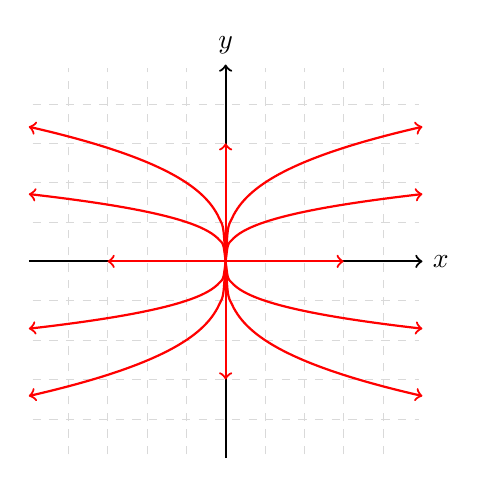
\begin{tikzpicture}[scale=0.5]
                \draw[help lines, color=gray!30, dashed] (-4.9,-4.9) grid (4.9,4.9);
                \draw[->,thick] (-5,0)--(5,0) node[right]{$x$};
                \draw[->,thick] (0,-5)--(0,5) node[above]{$y$};
                
                % Starts on axes
                \draw[red,->, thick] (0,0) -- (3,0);
                \draw[red,->, thick] (0,0) -- (-3,0);
                \draw[red,->, thick] (0,0) -- (0,3);
                \draw[red,->, thick] (0,0) -- (0,-3);
                
                % First Quadrant
                \draw[domain=-5:5, smooth, samples = 100, variable=\x, red, thick, <->] plot ({\x}, {\x^(1/3)});
                \draw[domain=-5:5, smooth, samples = 100, variable=\x, red, thick, <->] plot ({\x}, {2*\x^(1/3)});
                \draw[domain=-5:5, smooth, samples = 100, variable=\x, red, thick, <->] plot ({\x}, {-\x^(1/3)});
                \draw[domain=-5:5, smooth, samples = 100, variable=\x, red, thick, <->] plot ({\x}, {-2*\x^(1/3)});
                \end{tikzpicture}
        \end{center}
    \end{enumerate}
\end{sol}

\newpage

...and the second is
\begin{exercise}
    Let $A$ be diagonalizable matrix.
    \begin{enumerate}[label=(\alph*)]
        \item Show that the only solution to the system $\b{x}'=A\b{x},\, \b{x}(0)=\b{0}$ is the constant solution $\b{x}(t)=\b{0}$.
        \item Using part (a) show that if $\b{x}(t)$ and $\hat{\b{x}}(t)$ are two solutions to the system $\b{x}'=A\b{x},\, \b{x}(0)=\b{x}_0$, then $\b{x}(t)=\hat{\b{x}}(t)$.
    \end{enumerate}
\end{exercise}
\begin{sol}
    \begin{enumerate}[label=(\alph*)]
        \item $A$ is diagonalizable so we can write it as $A=SDS^{-1}$. If $y=S^{-1}x$, then it solves $y' = Dy$. If $x(0)=0)$, then $y(0) = S^{-1}x(0) = S^{-1}(0) = 0$ as well. However, $y' = Dy$ and since $y(0)=0$, this means that $y(t)=0$ for all $t$ (coefficients of general solution will all be zero).  
        \item \textbf{(Uniqueness of Solutions)}
    \end{enumerate}
\end{sol}
\end{document}
